%%%%%%%%%%%%%%%%%%%%%%%%%%%%%%%%%%%%%%%%%%%%%%%%%%%%%%%%%%%%%%%%%%% 
%                                                                 %
%                            CHAPTER                              %
%                                                                 %
%%%%%%%%%%%%%%%%%%%%%%%%%%%%%%%%%%%%%%%%%%%%%%%%%%%%%%%%%%%%%%%%%%% 

\chapter{Setting aanval}\label{sec:inferentieaanval}
Gedurende dit hoofdstuk wordt de setting alsook de werking van de aanval
beschreven. De aanval is sterk gebaseerd op de aanvallen
van~\citeauthor{Dhondt_Pochat_Voulimeneas_Joosen_Volckaert_2022}\cite{Dhondt_Pochat_Voulimeneas_Joosen_Volckaert_2022}
en~\citeauthor{Verdonck_2022}\cite{Verdonck_2022}. Deze aanvallen worden
inferentie-aanvallen genoemd, vanwege het feit dat uit metadata essentiële
gegevens kunnen worden geïnfereerd. In het geval
van~\citeauthor{Dhondt_Pochat_Voulimeneas_Joosen_Volckaert_2022} gaat dit over
afgelegde afstand binnenin de \ac{EPZ}. In het geval
van~\citeauthor{Verdonck_2022} gaat dit dan weer over geïnduceerde
hoogteverschillen binnen de privacy zone. Allereerst zal kort de mogelijkheden
van een aanvaller in de huidige setting worden besproken. Daarna wordt de
inferentie aanval
van~\citeauthor{Dhondt_Pochat_Voulimeneas_Joosen_Volckaert_2022}, die de basis
vormt voor de aanval in deze thesis, besproken volgens een opdeling in drie
stappen.

\section{Definitie aanvaller}
Deze thesis voert een onderzoek naar de mogelijkheid om een \ac{EPZ} te
omzeilen. De studie wordt dus gevoerd vanuit het opzicht van een aanvaller.
Vooraleer de werking van een aanval wordt beschreven, is het belangrijk om een
zicht te hebben op het doel, en de capaciteiten van een aanvaller.

Hier is een aanvaller een gebruiker van het platform, die geen eigenaar is van
een activiteit. Hij heeft echter wel zicht op alle metadata die publiekelijk
gedeeld zijn. Dit is data zoals afgelegde afstand, snelheid, tempo, \ldots
Aangezien de aanval gaat over het omzeilen \acp{EPZ} worden activiteiten
beschouwd die gecloaked zijn. De aanvaller heeft dus geen zicht op de reële
start- en/of eindlocatie, zijn doel is dan ook om ondanks de aanwezigheid van
cloaking deze gevoelige locatie te achterhalen.

Vanuit het oogpunt van de inferentie-aanval beschreven
door~\citeauthor{Dhondt_Pochat_Voulimeneas_Joosen_Volckaert_2022} heeft de
aanvaller toegang tot alle data die publiek beschikbaar is. Deze gebruikt dan
voornamelijk afgelegde weg als basis.

De aanvaller die in deze thesis wordt beschreven, heeft echter geen toegang tot
deze afstandsdata. Hij heeft wel nog toegang tot de ruwe GPS-data, maar ook de
snelheid, het tempo enzovoort. Het onderzoek bestaat er dus uit om te
onderzoeken in hoeverre een aanval nog mogelijk is wanneer de afstandsdata
onbruikbaar zou zijn. Een alternatieve aanpak wordt dus onderzocht om de
inferentie-aanval alsnog succesvol te kunnen uitvoeren.

\subsection{Assumpties}
Om de aanval te kunnen uitvoeren, moeten enkele assumpties worden gemaakt.
\citeauthor{Dhondt_Pochat_Voulimeneas_Joosen_Volckaert_2022} maakte al enkele
assumpties om de inferentie aanval succesvol uit te voeren. Voor dit onderzoek
moeten deze dus ook gelden. De eerste bestaat eruit opdat de zichtbare begin
-en eindpunten op de cirkel moeten liggen. Ten tweede moet de beschermde
locatie op de roadgraph liggen, hij kan niet buiten het voor ons te mappen
gebied liggen, bijvoorbeeld in een bos waar geen pad ligt. Er wordt dieper
ingegaan op de roadgraph in Sectie~\ref{sec:roadgraph}. Als laatste, maar
desalniettemin belangrijk punt moet de gebruiker binnenin de \ac{EPZ} de
kortste route volgen.~\cite{Dhondt_Pochat_Voulimeneas_Joosen_Volckaert_2022}

Dhondt et al.\ maakt nog een laatste assumptie over start- en eindpunten, die
hetzelfde moeten zijn. Dit is echter niet van toepassing op dit onderzoek. Het
onderzoek focust zich op activiteiten waar slechts één deel van het traject
gecloaked is. Dit wil dan ook zeggen dat de gebruiker ofwel vertrekt op de
gevoelige locatie, of er eindigt, maar niet beide. Op
Figuur~\ref{fig:totalDistanceAttack} zijn de 2 mogelijke scenarios van een
total distance attack terug te vinden, namelijk waarbij zowel gestart als
geëindigd wordt binnenin de zone. Dit wordt ook een \textit{total distance
    attack} genoemd, omdat enkel de totale afstand en de afstand buiten de \ac{EPZ}
nodig is. Op deze figuur zijn de rode punten gelabeld \textit{Start} en
\textit{End} de zichtbare start- en eindpunten. Dit scenario stelt dat één van
de reële start- of eindpunten de gevoelige locatie is, aangeduid met de zwarte
markering. Een andere aanval is de \textit{inner distance attack}, hierbij
zullen zowel de start als het einde van een activiteit binnenin het te
verbergen gebied liggen, dit is te zien op Figuur~\ref{fig:innerDist}. De
kennis van de afzonderlijke afstand die de gebruiker aflegt van de start tot de
rand van de \ac{EPZ} en van de rand van de \ac{EPZ} tot de eindlocatie is dan
ook een vereiste. Op de Figuur is opnieuw de zichtbare randpunten aangeduid in
het rood. Echter zal het onzichtbare traject voor beide gevallen doorlopen en
eindigen op de gevoelige locatie, wat in dit geval de reële start- en
eindlocatie is. In Sectie~\ref{sec:berekeningen} wordt dieper ingegaan op de
reden waarom een \textit{inner distance attack} niet mogelijk is. In deze
thesis worden dus alle activiteiten enkel een verhulde start- of eindlocatie
behouden, de rest wordt gefilterd in deze context.
\begin{figure}[h]
    \centering
    \begin{subfigure}[b]{.5\textwidth}
        \centering
        \caption{Start binnenin de \ac{EPZ}}
        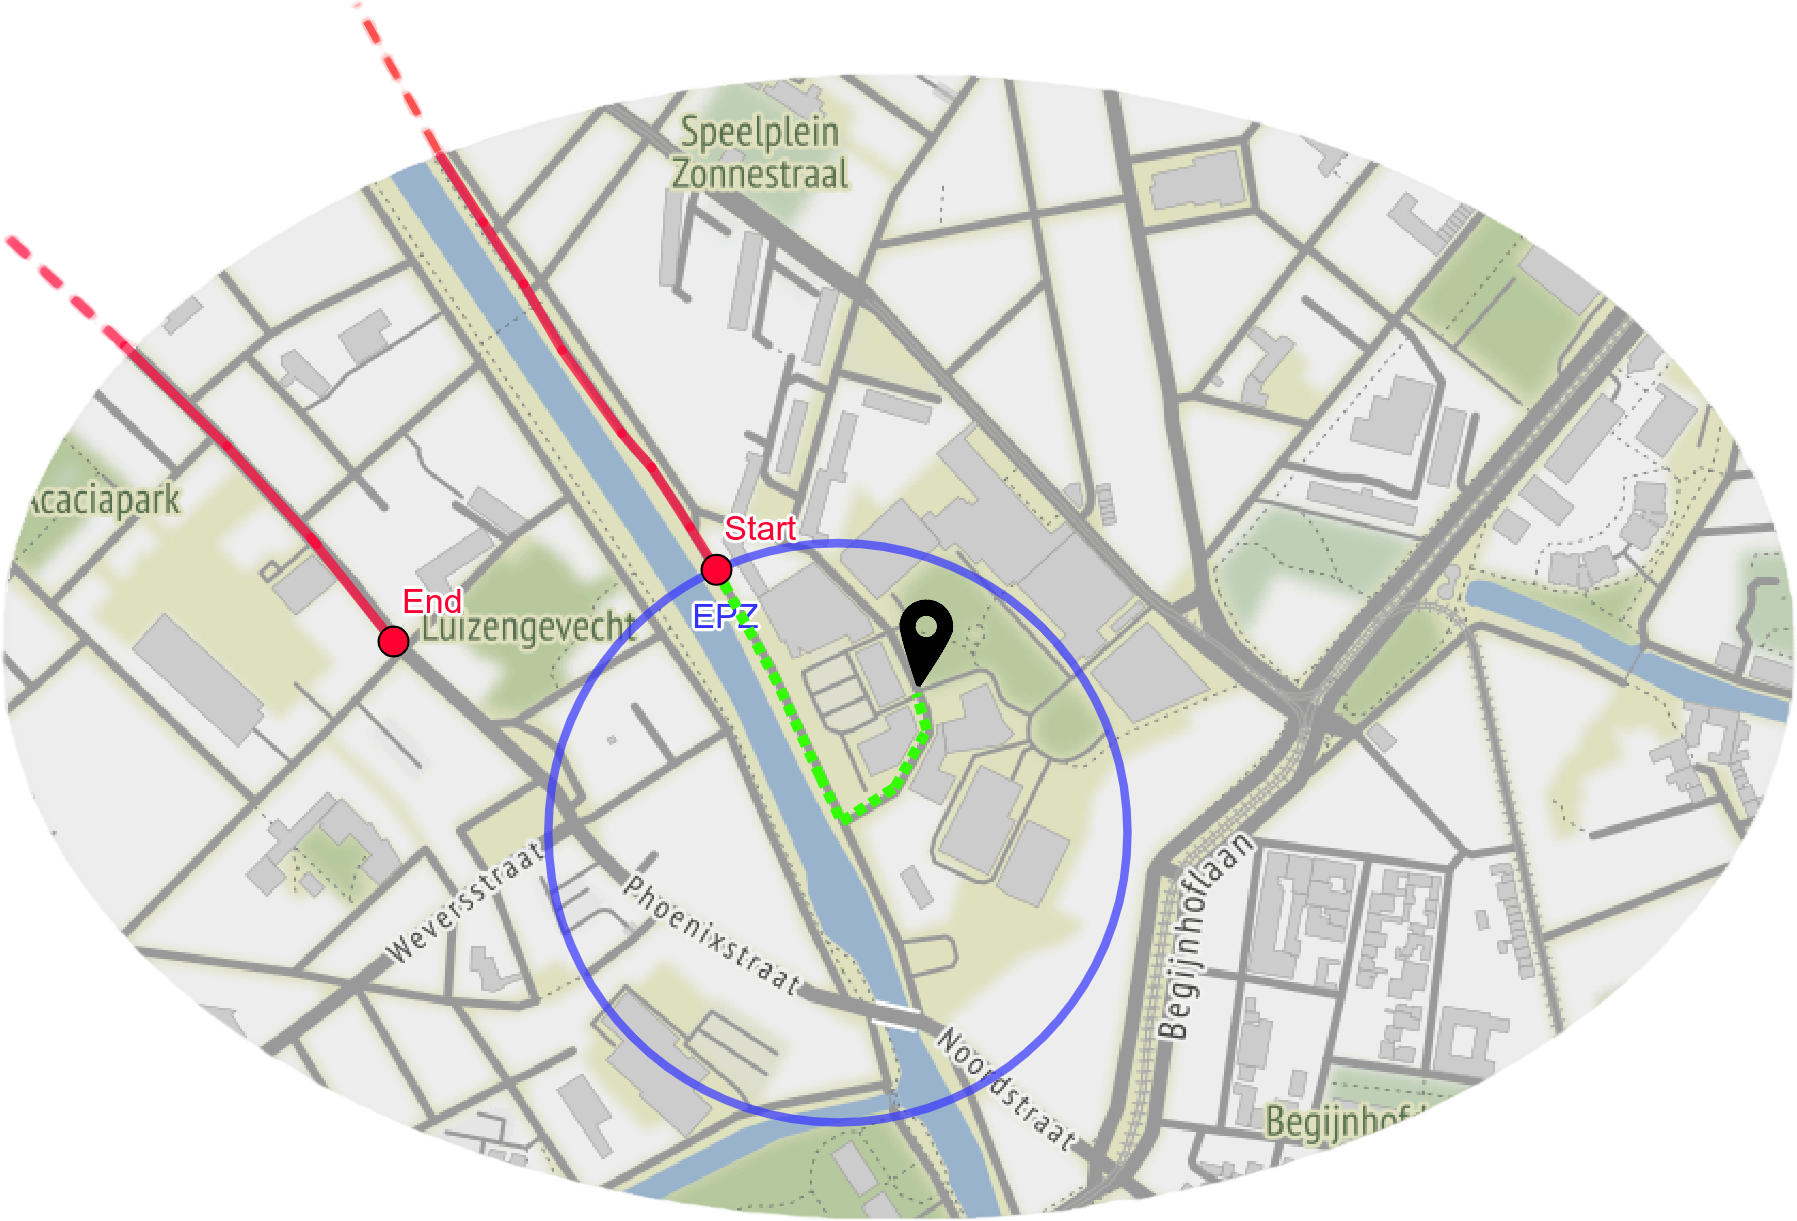
\includegraphics[width=1\textwidth]{fig/TotalDistanceAttacks/start.png}
    \end{subfigure}\hfill
    \begin{subfigure}[b]{.5\textwidth}
        \centering
        \caption{Einde binnenin de \ac{EPZ}}
        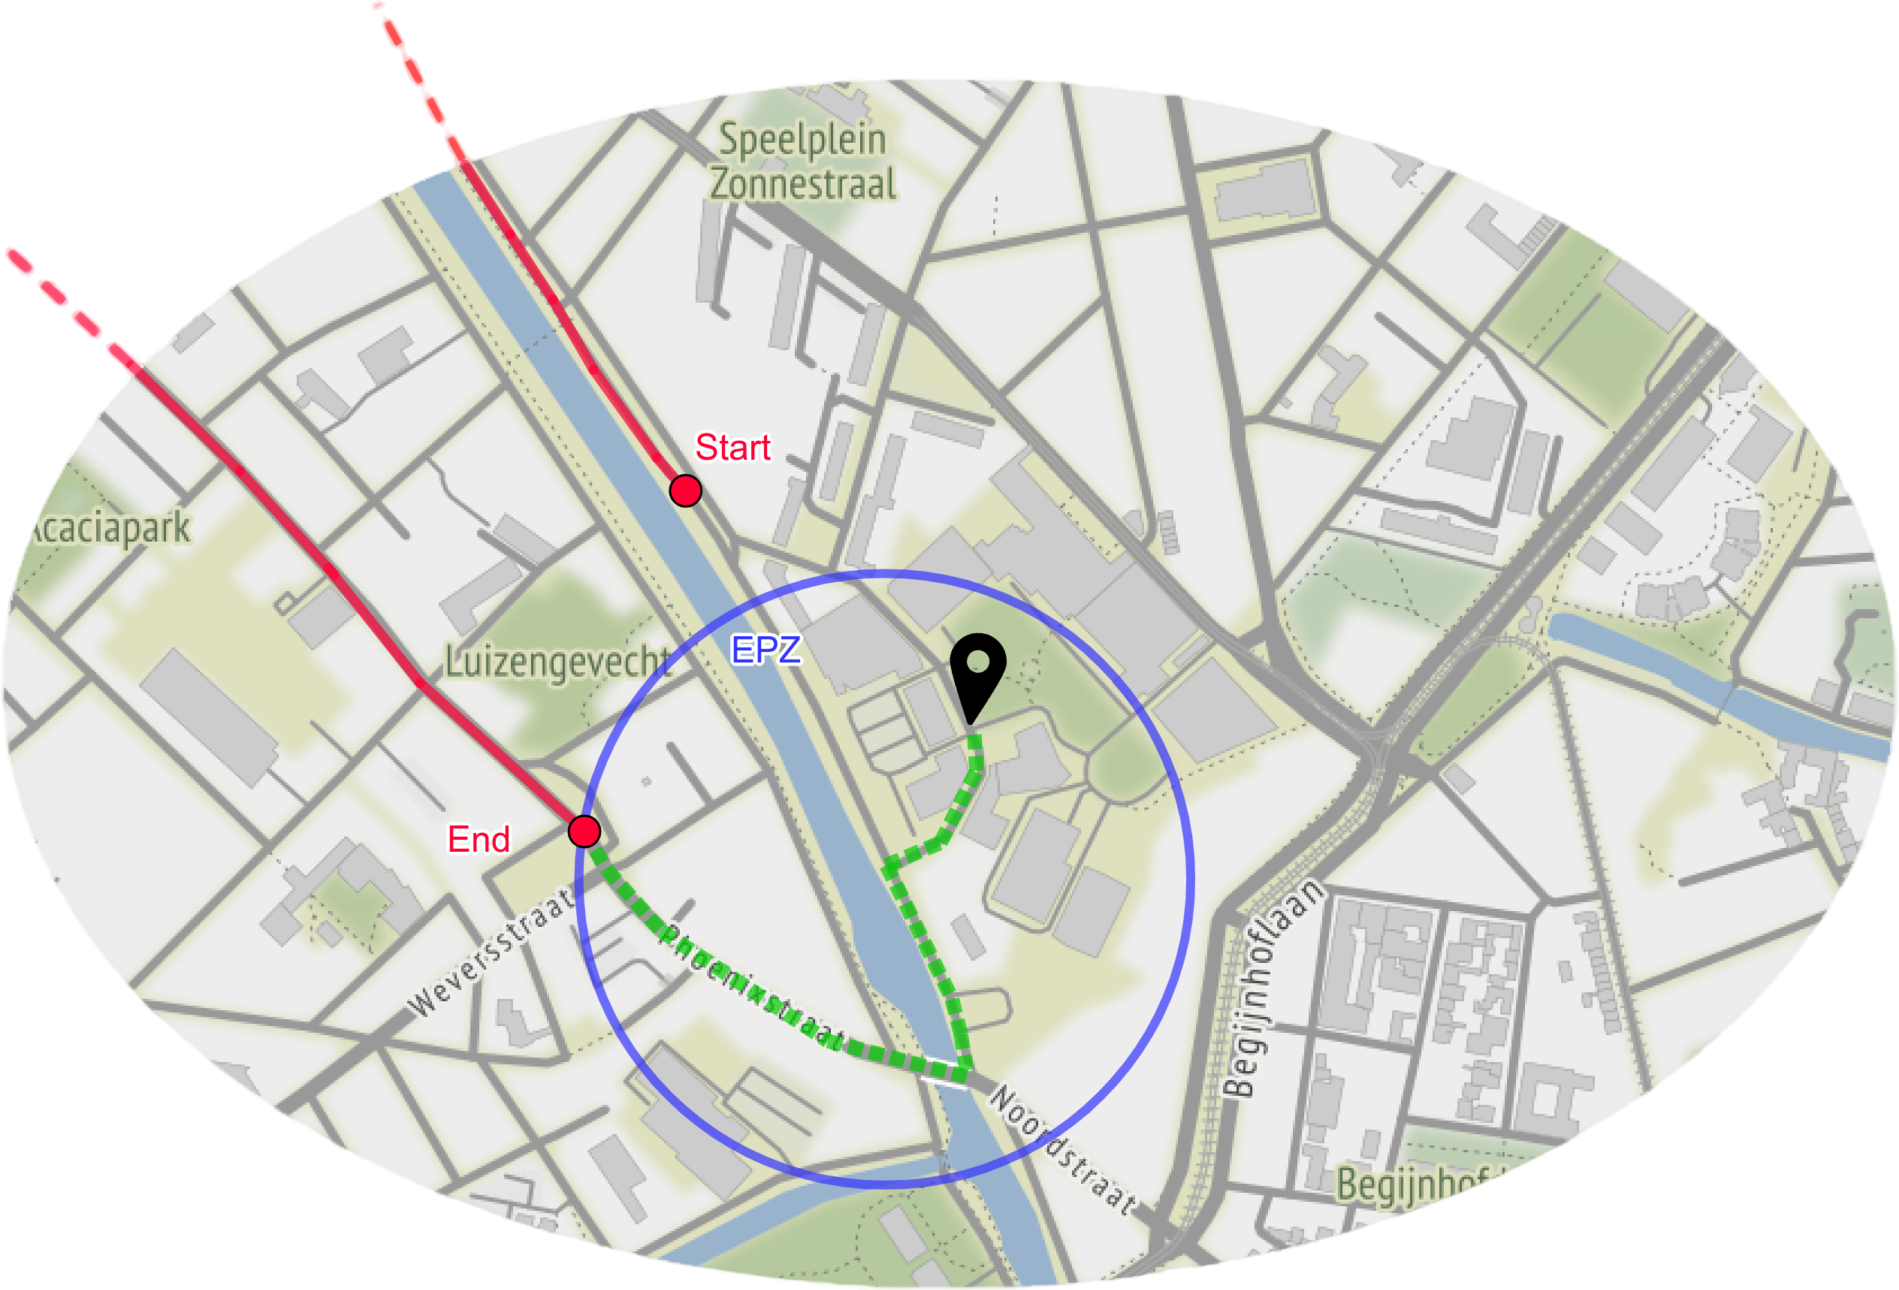
\includegraphics[width=1\textwidth]{fig/TotalDistanceAttacks/end.png}
    \end{subfigure}
    \caption{Voorbeeld van de mogelijke scenarios bij een total distance attack scenario}\label{fig:totalDistanceAttack}
\end{figure}
\begin{figure}[h]
    \centering
    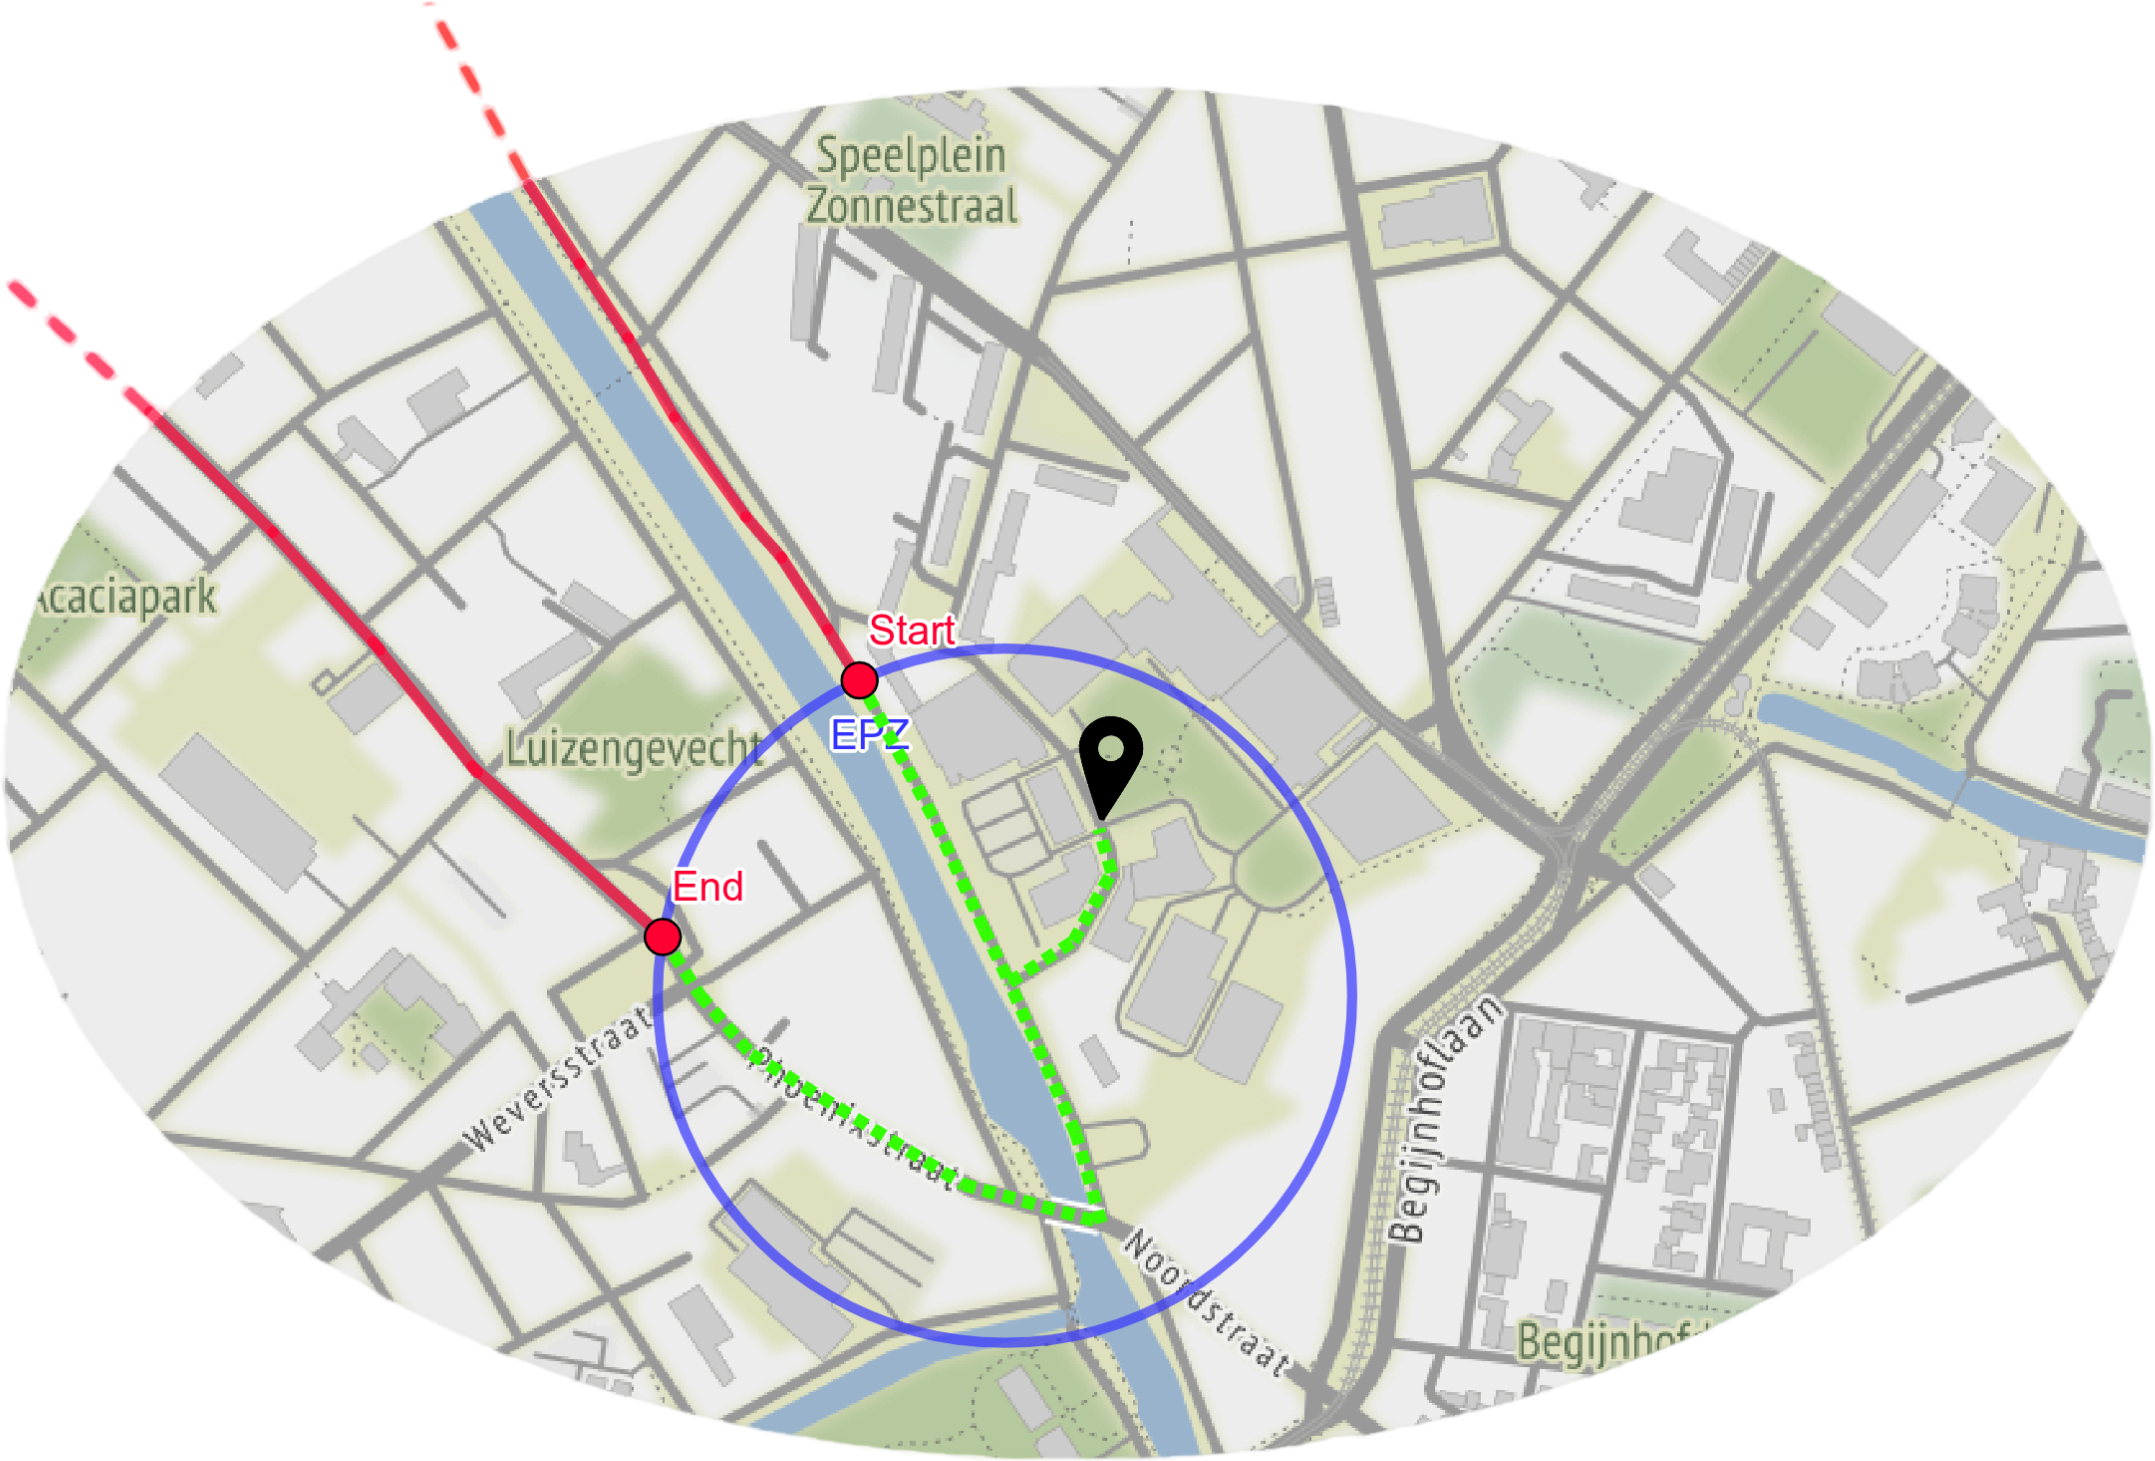
\includegraphics[width=.5\textwidth]{fig/TotalDistanceAttacks/InnerDistanceAttack.png}
    \caption{Voorbeeld van een inner distance attack situatie}\label{fig:innerDist}
\end{figure}

Deze thesis baseert zich ook voor een stuk op gemiddelde snelheden en tempo's.
Hierdoor stellen we volgende bijkomende assumptie voor: Een gebruiker mag niet
stilstaan binnenin de \ac{EPZ}. Platformen zoals Strava hebben namelijk een
ingebouwde functie die bij het uploaden van een activiteit tijden waarbij een
gebruiker stilstaat aan bijvoorbeeld een rood licht filtert. Zo kunnen ze een
meer representatieve gemiddelde snelheid en tempo berekenen en weergeven. Dit
wil wel zeggen dat de totale bewegingstijd waarop de gemiddelde snelheid en
tempo gebaseerd zijn, niet overeenkomt met de totale tijd van de activiteit.
Bij een berekening gebaseerd op totale verstreken tijd zou een significante
fout kunnen optreden.

\section{Identificeren van de EPZ}
De eerste hiervan is het identificeren van de \ac{EPZ}. Alhoewel deze stap niet
noodzakelijk is, vernauwt deze de zoekruimte drastisch. Hierbij worden van alle
activiteiten die van een gebruiker ter beschikking zijn gesteld, de zichtbare
begin- en eindpunten genomen. Deze zullen dan via k-means clustering worden
gegroepeerd opdat ze de zogenaamde \textit{entry gates} zullen aantonen.

K-means clustering is een unsupervised machine learning techniek die veel wordt
gebruikt bij het clusteren van data. Het is een iteratief proces waarbij het
algoritme $k$ clusters tracht te creëren waarbij de datapunten in elke cluster
zo dicht mogelijk bij het gemiddelde van die cluster
liggen~\cite{Understa24:online}. Dit algoritme kiest willekeurig initiële
middelpunten voor de verschillende clusters. Daarna worden alle punten in de
data toegekend aan de cluster met de laagste Euclidische afstand tot het
centrum van deze cluster. Daarna worden de gemiddeldes van deze clusters
herberekend, en worden deze gezien als nieuwe centrums. Opnieuw worden alle
punten aan de correcte cluster toegekend, en het proces wordt verschillende
iteraties herhaald tot een ietwat stabiele cirkel bekomen wordt. In de
implementatie van~\citeauthor{Dhondt_Pochat_Voulimeneas_Joosen_Volckaert_2022}
waarop deze thesis gebaseerd wordt, is een cirkel stabiel wanneer het verschil
in afstand tussen twee opeenvolgende gevonden cirkels kleiner is dan een
drempelwaarde, in dit geval 10
meter\cite{Dhondt_Pochat_Voulimeneas_Joosen_Volckaert_2022, Verdonck_2022}. Op
Figuur~\ref{fig:kmeans} is te zien hoe de clustering bij elke iteratie beter
wordt. In de context van het identificeren van de \ac{EPZ} zal het gebruikt
worden om \ac{gps}-punten te groeperen op basis van hun locaties. Punten die
dezelfde entry gate representeren, zullen in dezelfde cluster terecht komen.

\begin{figure}[h]
    \centering
    \begin{subfigure}[b]{.33\textwidth}
        \centering
        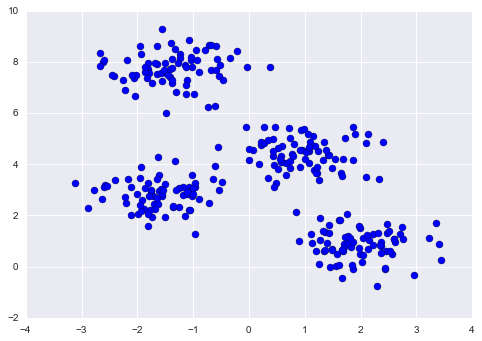
\includegraphics[width=1\textwidth]{fig/kmeans/1.png}
    \end{subfigure}\hfill
    \begin{subfigure}[b]{.33\textwidth}
        \centering
        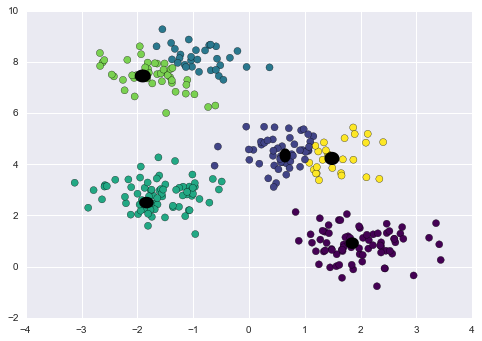
\includegraphics[width=1\textwidth]{fig/kmeans/2.png}
    \end{subfigure}
    \begin{subfigure}[b]{.33\textwidth}
        \centering
        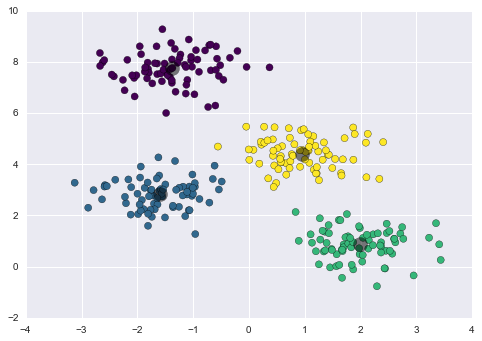
\includegraphics[width=1\textwidth]{fig/kmeans/3.png}
    \end{subfigure}
    \caption{Voorbeeld werking k-means clustering~\cite{InDepthk59:online}}\label{fig:kmeans}
\end{figure}

De besproken entry gates zijn zoals de naam al doet vermoeden de
`toegangspoorten' tot de cirkel. Dit is waar de gebruiker de \ac{EPZ} betreedt
en/of verlaat. Deze punten zouden dus in theorie de \ac{EPZ} perfect moeten
definiëren. Maar door de fouten die standaard met het meten van gps-punten
komen\footnote{Gps-metingen bevatten standaard onnauwkeurigheden, er kan
    bouncing of signal loss voor een bepaalde interval optreden. Ook kan slechts op
    bepaalde tijdsintervallen de locatie worden genomen, perfect op de cirkel kan
    dus nooit gemeten worden.} is dit niet perfect. Op Figuur~\ref{fig:entrygate}
is te zien dat meerdere eindpunten van activiteiten geclusterd worden tot één
\ac{E.G.}, op de figuur voorgesteld door een kruis. Een cirkel kan worden
gedefinieerd door drie punten, bijgevolg moeten er dus ten minste drie
\ac{E.G.} gevonden worden.
\begin{figure}
    \centering
    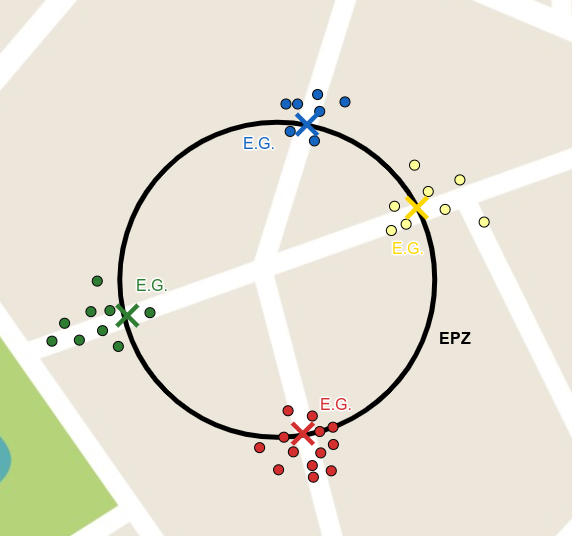
\includegraphics[width=0.5\linewidth]{fig/EPZ-mechanisme/Entry_Gate.png}
    \caption{Voorbeeld van entry gates gevonden door k-means clustering en identificatie van de \ac{EPZ}}\label{fig:entrygate}
\end{figure}

Het algoritme zal na de identificatie van de \ac{EPZ} ook nog nakijken of er
niet meer dan één \ac{EPZ} te vinden is. Er wordt onderzocht of punten die
meegenomen zijn in de beschouwing van de huidige \ac{EPZ}, toch niet horen bij
een mogelijke andere \ac{EPZ} van de user. Als controle wordt van elk eind- of
beginpunt de Euclidische afstand berekent tot de rand van de bijhorende
gevonden \ac{EPZ}. Indien deze kleiner is dan de grootst mogelijke radius, dan
wordt verondersteld dat het punt bij deze zone hoort. Indien dit voor alle
punten geldt, dan stopt het algoritme hier. In het andere geval waarbij de
berekende afstand groter is, worden meer clusters toegevoegd aan het algoritme
van k-means clustering. Dit zal dus een nieuwe privacy zone aanwijzen.

Deze stap is niet noodzakelijk in het globale verhaal van de thesis, maar is
wel een stap die de zoekruimte erg kan verkleinen. Indien het algoritme één of
meerdere \acp{EPZ} vindt, dan zullen er enkel voorspellingen gebeuren in de
regio binnenin. Indien dit niet het geval is en er geen \ac{EPZ} gevonden is,
bestaat de kans dat voorspellingen van locaties gebeuren buiten de verhullende
zone. Ook is in dit geval een groter stuk van het stratenplan nodig om de
locatie te achterhalen.

\section{Bepalen nodige gegevens voor predictie}
Na de bepaling van de \acp{EPZ} voor de gebruiker wordt overgegaan tot het
berekenen en achterhalen van de bijhorende gegevens die nodig zijn om de
gevoelige locatie te voorspellen. Hiervoor wordt verder ingegaan op de
methodiek in de
paper~\citeauthor{Dhondt_Pochat_Voulimeneas_Joosen_Volckaert_2022}, maar er
worden enkele gegevens op een andere manier benadert volgens de huidige
definitie van de aanvaller.

\subsection{Roadgraph en Distance Matrix}\label{sec:roadgraph}
Voor elke gevonden EPZ is het noodzakelijk om een graafvoorstelling van de
omgeving op te stellen. Op Figuur~\ref{fig:graph_generation} is een voorbeeld
terug te vinden van hoe een graaf kan worden geëxtraheerd. Er worden punten
geplaatst op de straten op een vaste afstand van elkaar, en deze kunnen dan
worden verbonden. Indien geen \acp{EPZ} geïdentificeerd zijn, dan wordt de
omgeving die moet worden omgezet naar een graaf een stuk ruimer genomen. De
graafvoorstelling bestaat uit een serie van nodes, die zich allemaal op een
gekende straat bevinden. De bogen waarmee de nodes verbonden zijn, volgen het
straatplan, opdat een node een mogelijks te volgen weg
is~\cite{neira2022graph}. Aan de hand van de `Chaining Distance' wordt bepaald
hoeveel afstand tussen de nodes zal zitten, en zo dus impliciet ook welke
densiteit het netwerk zal hebben. Hoe lager de densiteit, hoe meer nodes, en
dus ook hoe preciezer. Om voorspellingen te maken is wel een bepaalde precisie
vereist, dus mag deze waarde niet te hoog zijn. Empirisch werd gekozen voor een
waarde van $3.0m$.
\begin{figure}[h]
    \caption{Voorbeeld van het genereren van een roadgraph}\label{fig:graph_generation}
    \centering
    \begin{subfigure}[b]{.4\textwidth}
        \centering
        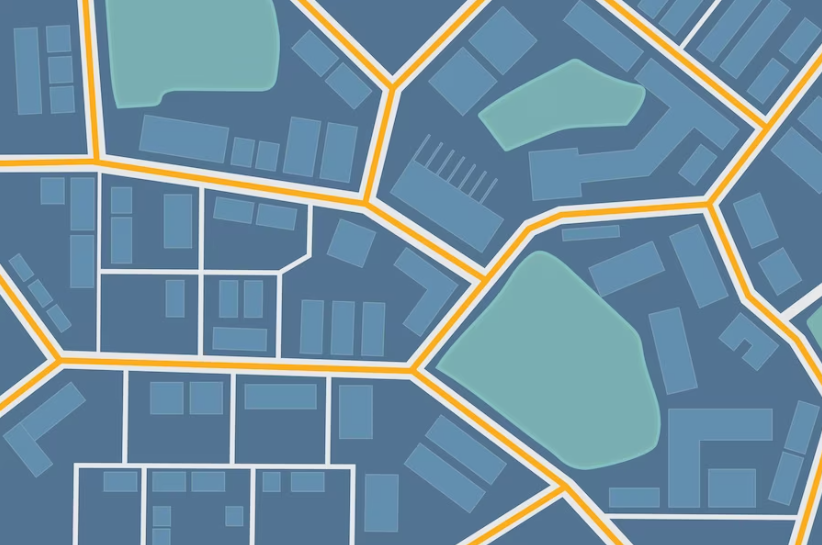
\includegraphics[width=1\textwidth]{fig/RoadGraph/RoadMap.png}
        \caption{Voorbeeld stratenplan}
    \end{subfigure}\hfill
    \begin{subfigure}[b]{.4\textwidth}
        \centering
        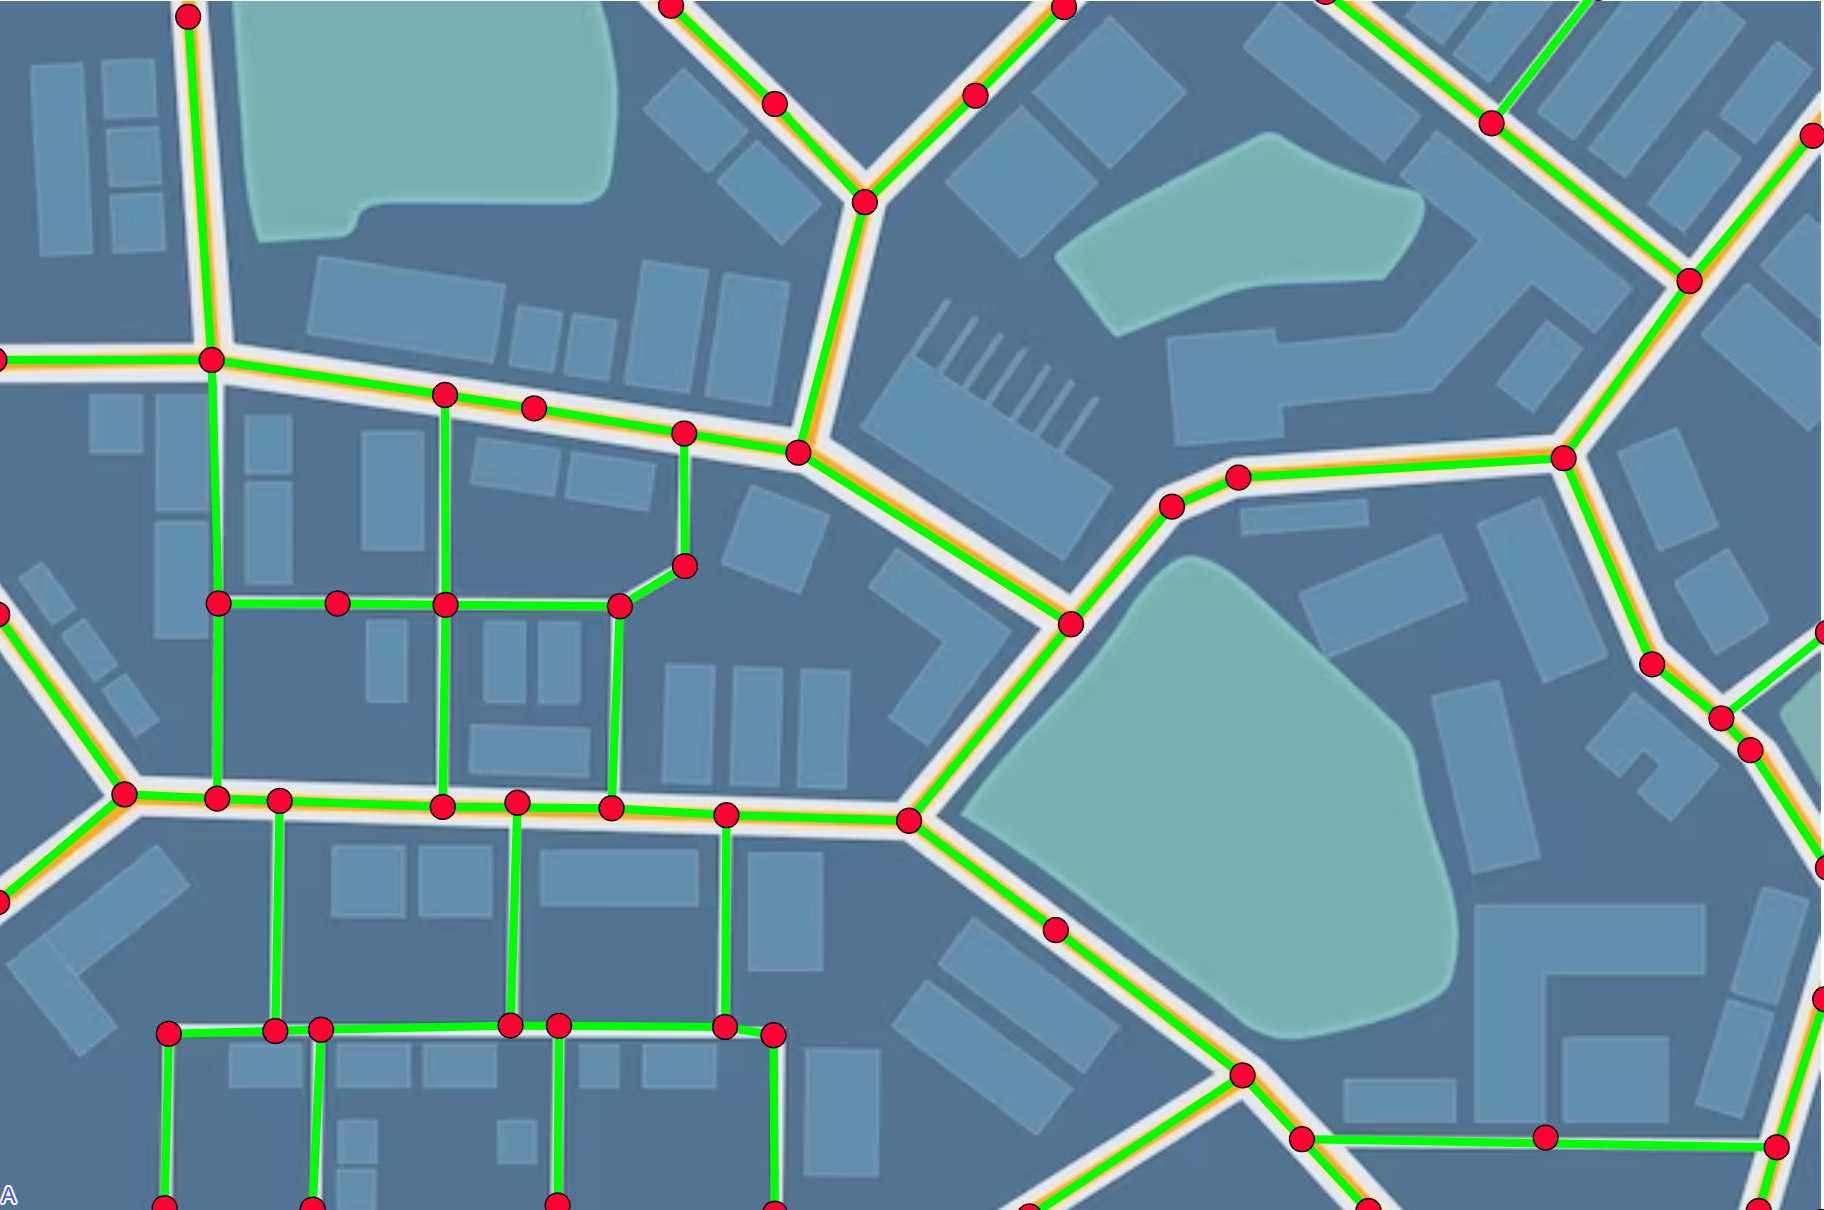
\includegraphics[width=1\textwidth]{fig/RoadGraph/Graph_Over_Map.png}
        \caption{Nodes en bogen geplot op het stratenplan}
    \end{subfigure}
    \begin{subfigure}[b]{.4\textwidth}
        \centering
        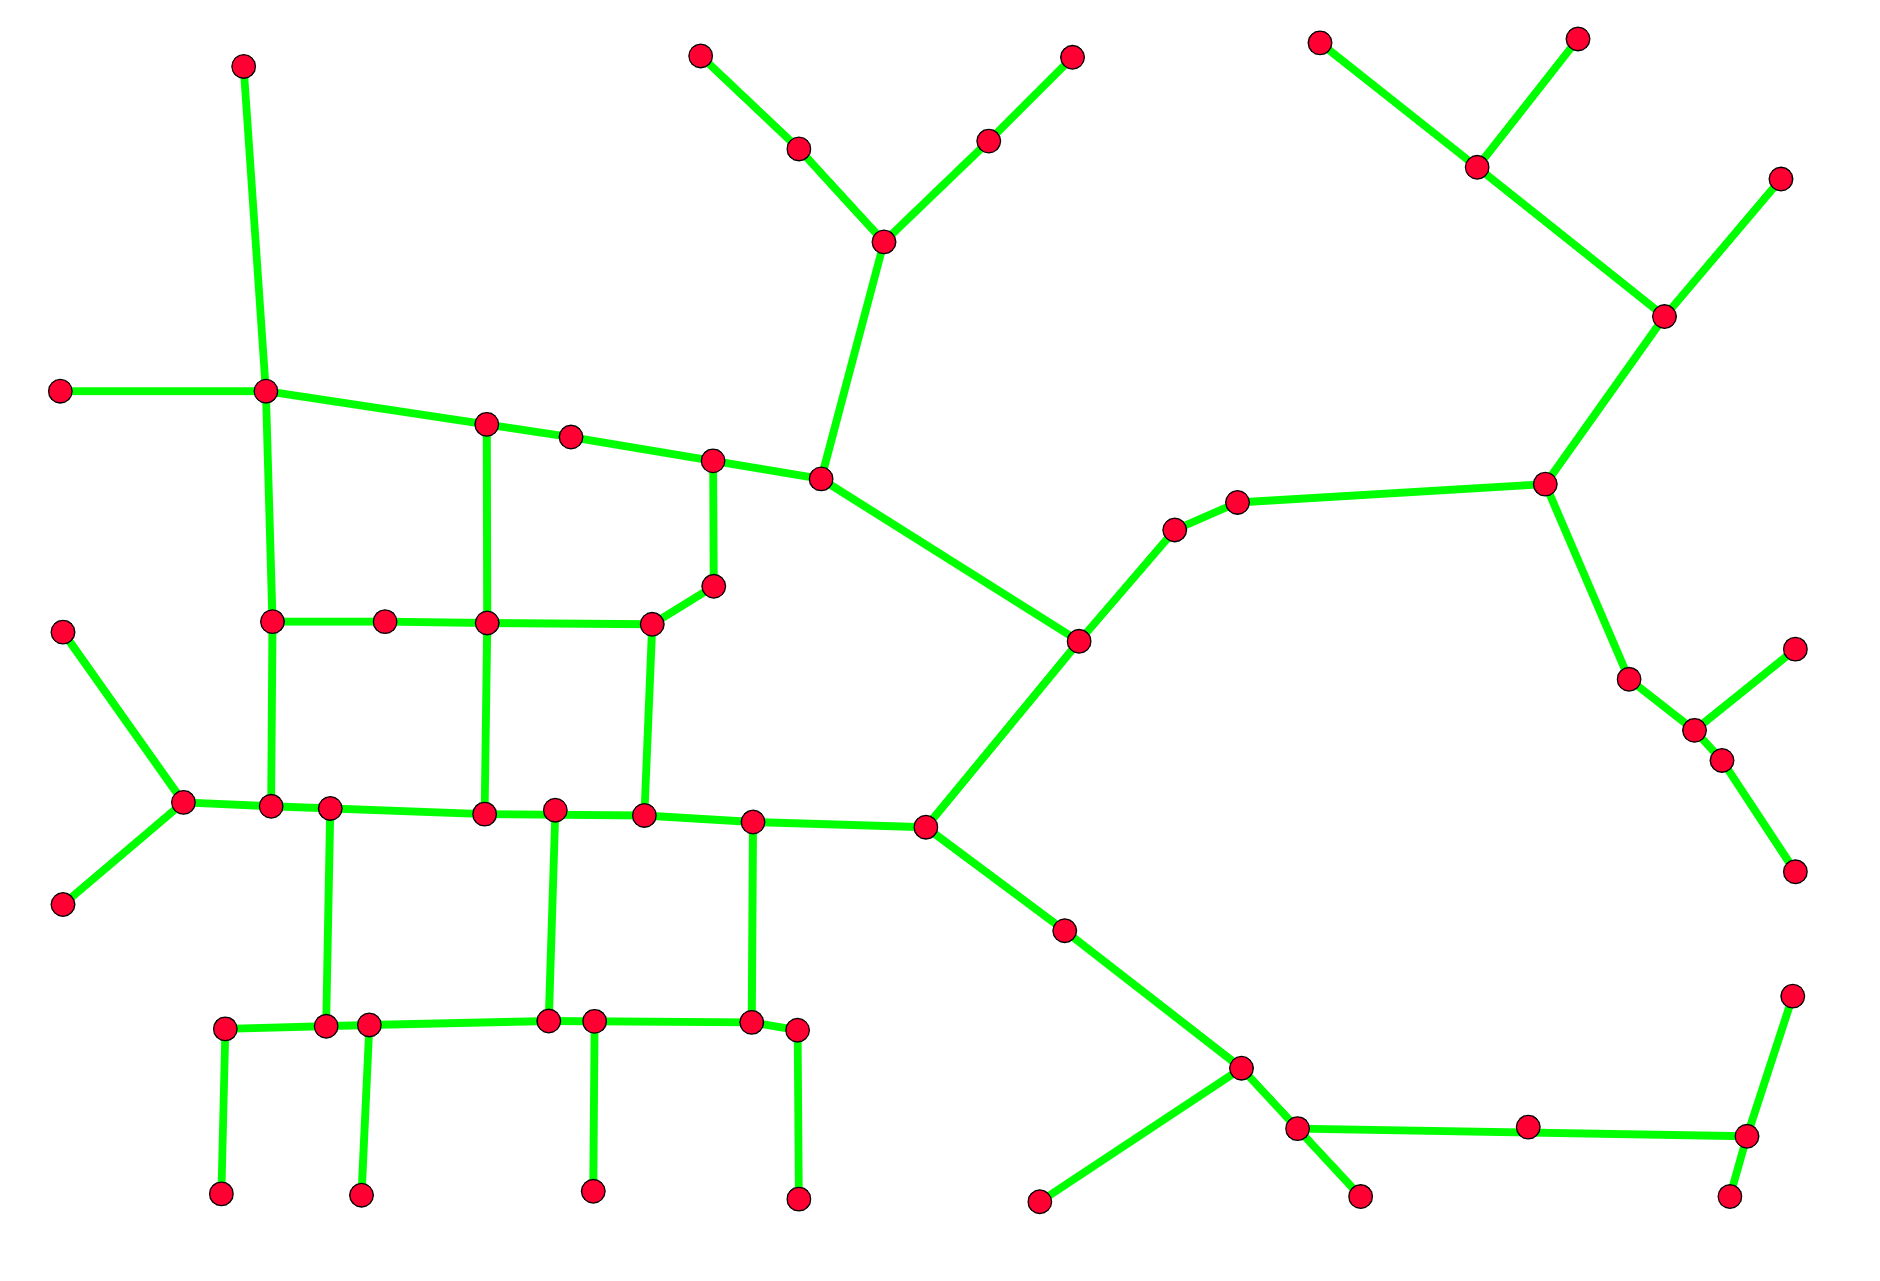
\includegraphics[width=1\textwidth]{fig/RoadGraph/Graph.png}
        \caption{Resulterende graafvoorstelling van het stratenplan}
    \end{subfigure}
\end{figure}

Op basis van de nodes in deze graaf, kan de \textit{Distance Matrix} worden
opgesteld. Dit is een matrix die voor alle startnodes (op de rand van de
\ac{EPZ}) de theoretische afstand bevat tot alle nodes aanwezig in de graaf.
Gebruikmakend van het Dijkstra algoritme\footnote{Het Dijkstra-algoritme is een
    algoritme in de grafentheorie dat wordt gebruikt om de kortste weg te vinden
    tussen twee knooppunten in een gewogen grafiek. Het algoritme werkt door
    iteratief knooppunten toe te voegen aan een `bezochte' set en de kortste
    afstand te berekenen vanaf het beginpunt naar elk aangrenzend knooppunt dat nog
    niet is bezocht\cite{dijkstra}.}, die het in staat stelt om voor elk punt de
kortste theoretische afstand te bepalen tot alle punten in de graaf. Deze
afstanden worden opgeslagen, en zijn belangrijk in een verder stadium van de
aanval.

\subsection{Begin- en eindnodes}
Voor elke activiteit is het volledige traject buiten de \ac{EPZ} gegeven. Dit
omvat alle \ac{gps}-punten die niet verborgen zijn. De begin- en eindnodes van
het traject zijn hier van belang. Voor de duidelijkheid en de vlotheid van de
tekst zullen we naar deze punten refereren als het zichtbare beginpunt en het
zichtbare eindpunt. Volgens één van de voorafgaand gemaakt assumptie vertrekt
of eindigt de sporter in de \ac{EPZ}. Dit betekent dat ofwel het reële
eindpunt, ofwel het reële beginpunt zal overeenstemmen met de gevoelige
locatie. In geval dat een gebruiker aankomt binnenin de \ac{EPZ}, en dus ook
vertrekt erbuiten, starten de berekeningen vanaf het zichtbare eindpunt. En
omgekeerd, indien hij vertrekt binnenin de \ac{EPZ}, worden de berekeningen
gestart vanaf het zichtbare beginpunt. Deze punten zullen in het vervolg
\textit{randpunten} genoemd worden, refererend naar de rand van de \ac{EPZ}.
Deze \textit{randpunten} zullen de basis vormen voor de volgende berekeningen.

Bijhorend zijn bij de randpunten ook bepaalde extra gegevens beschikbaar. De
belangrijkste zijn de cumulatieve afstand tot dit punt\footnote{De totale
    afstand afgelegd vanaf het begin van de activiteit tot en met het punt in
    kwestie.}, en de cumulatieve tijd tot dit punt\footnote{De totale afstand
    afgelegd vanaf het begin van de activiteit tot en met het punt in kwestie.}.
Bij de aanval van Dhondt et al.\ wordt de afstand gebruikt om predicties t
doen, dit wil dus zeggen dat deze afstand dus aan de basis zal liggen. Maar in
deze thesis wordt ervan uitgegaan dat afstanden verborgen worden. Onder het
verbergen van afstanden wordt een onderscheid gemaakt tussen 2 scenarios: het
eerste gaat ervan uit dat de totale afstand verborgen wordt, maar de
cumulatieve afstand gegeven is. Het tweede scenario gaat ervan uit dat alle
afstandsgegevens verborgen worden. Het alternatieve type data waar dus mee zal
moeten gewerkt worden is dus \ac{gps}-data.

\subsection{Berekeningen afstand binnenin de EPZ}\label{sec:berekeningen}
Om voorspellingen te kunnen doen zullen volgens de inferentie aanval die hier
besproken wordt twee belangrijke gegevens ter beschikking moeten zijn. Met name
het straatnetwerk met de mogelijks gevolgde routes, wat werd besproken in
Sectie~\ref{sec:roadgraph}, en de afstand die wordt afgelegd binnenin de
\ac{EPZ}. Deze afstand benoemen we ook als de \textit{inner distance}.

In de implementatie
van~\citeauthor{Dhondt_Pochat_Voulimeneas_Joosen_Volckaert_2022} kan de
\textit{inner distance} simpelweg berekent worden door het verschil te nemen
tussen de afgelegde afstand buiten de verhulde zone (deze noemen we de
\textit{outer distance}), en de totale afstand: \[inner\ distance = total\
    distance - outer\ distance \]

In deze thesis moet dit echter gebeuren met een tussenstap. In het eerste
scenario waarbij de cumulatieve afstand gegeven is, maar de totale afstand
niet, moet de totale afstand berekend worden. Maar door de aanwezigheid van
snelheid- en tijdsgegevens kan dit via basisformules gebeuren. Gebruik makend
van het gemiddelde tempo kan de voorgaande formule worden omgevormd tot: \[inner\ distance = total\ time \times average\ pace - outer\ distance \]

In opzicht van het tweede scenario, waarbij alle afstandsgegevens verborgen
zijn, ontbreekt nu ook de \textit{outer distance}. We bepalen deze dan ook via
de \ac{gps}-coördinaten. Dit gebeurd door de som te nemen van de afstanden van
alle opeenvolgende punten. Let wel dat we de afstand tussen twee
\ac{gps}-punten berekenen gebruik makend van de \textit{haversine} formule.
Equation~\ref{eq:haversine} is een uitwerking van de formule. Deze berekent de
afstand tussen twee punten op een bolvormig oppervlak, in dit geval de aarde.
Om de afstand tussen twee punten op het aardoppervlak te berekenen, moeten de
breedte- en lengtegraden van elk punt worden omgezet naar radialen. Vervolgens
worden deze waarden ingevoerd in de formule, samen met de straal van de aarde
($r$), meestal genomen als $6.371 km$. De formule berekent dan de haversine van
de helft van het verschil tussen de breedtegraden en de haversine van de helft
van het verschil tussen de lengtegraden ($\lambda$), evenals de cosinus van de
breedtegraden ($\phi$) van beide punten. Deze waarden worden vervolgens
gebruikt om de afstand tussen de twee punten te berekenen tussen de punten P \&
Q op Figuur~\ref{fig:haversine}~\cite{sheppard1922practical}.

Merk op dat ook dit een benadering is van de werkelijke afstand. De aarde is
niet perfect sferisch, wat de nauwkeurigheid kan beïnvloeden. Maar voor de
doeleinden van deze thesis is dit voldoende nauwkeurig, zeker omdat de
afstanden in deze context relatief klein zijn, waardoor over het algemeen
slechts een minimale buiging is.
\begin{equation}\label{eq:haversine}
    d = 2r \arcsin\left(\sqrt{\sin^2\left(\frac{\phi_2-\phi_1}{2}\right)+\cos(\phi_1)\cos(\phi_2)\sin^2\left(\frac{\lambda_2-\lambda_1}{2}\right)}\right)
\end{equation}
\begin{figure}[h]
    \centering
    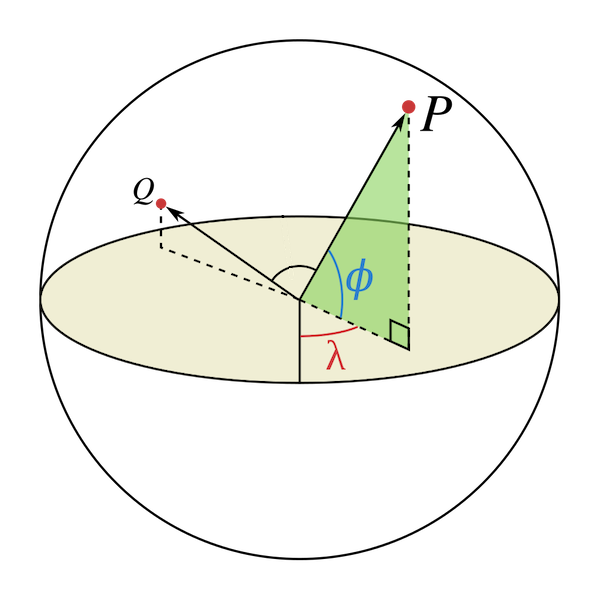
\includegraphics[width=0.5\textwidth]{fig/haversine.png}
    \caption{Haversine illustratie voor het berekenen van de afstand\cite{Distance97:online}}\label{fig:haversine}
\end{figure}

Uit de voorgaande paragrafen kunnen we dus besluiten dat de inner distance af
te leiden valt uit gegeven outer distance, total time en de gemiddelde
snelheid. Om een \textit{outer distance attack} uit te voeren is de berekening
van de totale inner distance voldoende. Maar bij het uitvoeren van een
\textit{inner distance attack} zijn twee aparte inner distances nodig (degene
van start tot de \ac{EPZ} en degene van de \ac{EPZ} tot de finish). Wanneer de
cumulatieve afstand gegeven is, zouden we een deze aanval kunnen uitvoeren
doordat in dit geval de twee afstanden te achterhalen zijn. $d_{start} =
    d_{eerste\ node}$ en $d_{finish} = d_{totaal} - d_{laatste\ node}$. Maar
wanneer deze niet beschikbaar zijn, is dit niet mogelijk, in dit geval zijn
deze afstanden niet individueel te achterhalen.

\section{Voorspellen locatie}
Alle nodige gegevens zijn nu beschikbaar om de gevoelige locatie te
achterhalen. Hier wordt besproken hoe voor elke bruikbare activiteit een
locatie zal worden voorspeld. Doordat voor elke activiteit één of meerdere
locaties worden voorspeld, zullen deze moeten worden gebundeld tot één locatie,
voor alle activiteiten.

\subsection{Filteren activiteiten}
Voorafgaand aan het voorspellen van de locatie, is het belangrijk dat enkel
voorspellingen gebeuren met activiteiten die een nuttige voorspelling kunnen
voortbrengen. De andere activiteiten zouden enkel de accuraatheid van de
voorspelling naar beneden halen. Dit gaat dan over activiteiten waarbij niet de
kortste route binnenin de \ac{EPZ} wordt gevolgd. Al deze activiteiten proberen
we dus in de mate van het mogelijke eruit te filteren.

Het geval waarbij een gebruiker niet de kortste route volgt vanaf de rand van
de \ac{EPZ} tot de gevoelige locatie kan in zekere mate worden opgevangen door
te stellen dat een activiteit enkel wordt gebruikt wanneer de nog af te leggen
afstand binnenin de \ac{EPZ} kleiner dan de maximaal mogelijk af te leggen weg.
In de andere gevallen zal de activiteit worden gefilterd. De maximale afstand
die hiervoor nodig is wordt bepaald gebruik makend van de \textit{Distance
    Matrix}, die beschreven staat in Sectie~\ref{sec:roadgraph}. De maximale
afstand is gelijk aan de maximale afstand terug te vinden in de matrix, voor de
bijhorende startnode. Dit is de afstand die een gebruiker maximaal kan afleggen
naar eender welke node op de graaf, vertrekkend van de startnode, door het
volgen van de theoretisch kortste route. Dit zal ook voor een stuk gevallen in
rekening brengen waarbij de activiteit voor een stuk verborgen wordt, maar niet
zal eindigen op de gevoelige locatie.

Op een gelijkaardige manier kan een filtering gebeuren voor afgelegde afstanden
die lager zijn dan de minimale mogelijke afstand. Dit zou opnieuw activiteiten
kunnen filteren die niet eindigen op de gevoelige afstand. De minimale afstand
is dan ook degene tot de node met de laagste minimale afstand tot deze node
vanaf het zichtbare startpunt/eindpunt van de activiteit, gelegen op de rand
van de \ac{EPZ}.

Ook worden de zichtbare eind- en beginpunten van de activiteiten gecontrolleerd
naar compatibiliteit met de road graph. Alle eind- en beginpunten worden
gesnapt op de roadgraph. Ze worden dus vervangen door de dichtstbijzijnde node
op de graaf. Indien het verschil in afstand tussen de originele locatie en de
gesnapte locatie te groot is, wordt de activiteit gefilterd. Dit wijst dan op
een te grote afwijking tussen de activiteit en de road graph, of op inaccurate
gps-data.

Als laatste wordt ook nog gekeken naar afwijkingen bij de \acp{E.G.}. Indien
bij het bepalen van een \acp{E.G.} een afwijking wordt vastgesteld tussen de
verschillende gebruikte endpoints/startpoints, die groter is dan drie maal de
standaardafwijking, wordt de activiteit gefilterd. Dit wijst dan op een te
grote spreiding bij de entry gates, en dus op een grote kans op inaccurate
voorspellingen.

\subsection{Bepalen van de locatie}
Om een predictie te maken per activiteit wordt de inner distance die berekent
werd in Sectie~\ref{sec:berekeningen} gebruikt. Deze wordt dan gematched met
het stratennetwerk. Het idee hierachter is om een alle mogelijke routes
binnenin de \ac{EPZ} af te leggen (die de kortste route vormt naar de nodes op
het pad), en te stoppen wanneer de afgelegde afstand gelijk is aan de berekende
inner distance. Het resultaat van al deze routes is dan een node, die mogelijks
de gevoelige locatie kan zijn. In de praktijk kan dit mechanisme op een
simpelere manier worden toegepast door het gebruik van de voorafgaande distance
matrix. De berekende inner distance zal worden vergeleken met de afstand in de
distance matrix, en de nodes in de \ac{EPZ} die het dichtst bij deze afstand
liggen zullen worden geselecteerd als kandidaten voor de gevoelige locatie.
Indien dit proces herhaald wordt voor alle beschikbare activiteiten, met
mogelijks verschillende Entry Gates, zullen er verschillende kandidaten worden
gevonden. Ook zullen bepaalde nodes meer dan één keer worden voorspeld. In de
volgende stap zullen alle predicties worden samengenomen in één voorspelling.

\subsection{Meest voorspelde locatie}
Een verzameling van nodes is nu bekomen, die normaliter ook de gevoelige
locatie bevat. Om deze te bepalen, wordt regressie-analyse toegepast, aan de
hand van de \ac{LAD} methode. Het resultaat van deze regressie-analyse zal een
\ac{gps}-locatie zijn, die onze \textit{eindvoorspelling} zal vormen.

De \ac{LAD} methode wordt gebruikt om een lineaire regressie uit te voeren op
een set punten, door de som van de absolute waarden van de absolute verschillen
te minimaliseren.\ \ac{LAD} staat gekend als een robuuste methode die erg
nuttig blijkt te zijn voor datasets met grote uitschieters. In
Vergelijking~\ref{eq:LAD} is te zien dat, door het werken met absolute waarden
van de vergelijking staat afwijkingen tussen de waarden, de extremen in mindere
mate doorwegen in de berekeningen. Dit is een groot voordeel ten opzichte van
andere regressietechnieken, zoals
bijvoorbeeld~\ac{OLS}\cite{iqbal2021application}.~\ac{OLS} werkt gelijkaardig,
maar zoals te zien is in Vergelijking~\ref{eq:OLS} probeert de som van de
kwadratische afwijkingen te minimaliseren. Uitschieters zullen dus meer
doorwegen. Een nadeel van \ac{LAD} is dat het berekenen van de LAD-schattingen
meer rekentijd en computerbronnen vereist dan \ac{OLS}, wat het minder geschikt
maakt voor grote datasets.
\begin{equation} \label{eq:LAD}
    LAD:\indent  \min\sum\limits_{i=1}^n|y_i - \hat{y}|
\end{equation}
\begin{equation} \label{eq:OLS}
    OLS:\indent  \min\sum\limits_{i=1}^n{(y_i - \hat{y})}^2
\end{equation}

LAD regressie wordt in deze thesis door de aard van de data, en van de
voorspellingen, meer bepaald door de grote kans op uitschieters. Gps-data kan
erg onnauwkeurig zijn, en grote of kleine afwijkingen kunnen dus voorkomen. Ook
is het mogelijk dat door acties van een sporter zoals bijvoorbeeld eenmalig de
kortste route niet volgen een uitschieters voorvallen. Rekentijd is in deze
thesis geen probleem, aangezien het aantal voorspelde locaties beperkt.

In de context van deze thesis kan de Vergelijking~\ref{eq:LAD} worden toegepast
voor elke voorspelde locatie. Alle voorspelde locaties zullen worden beschouwd
als mogelijke \textit{eindvoorspelling}. Deze zal dan in de vergelijking
$\hat{y}$ voorstellen. De absolute waarde van het verschil tussen de
eindvoorspelling en alle punten zal worden opgeteld. Er wordt dan gezocht naar
de \textit{eindvoorspelling} die de som van de absolute waarden, en dit is dan
de resulterende predictie.